% ---------------------------------------------------------------------------
% Molecular Informatics (Wiley-VCH) -- Full Paper, manuscript-submission layout (v4)
% Compile with pdfLaTeX (twice) and BibTeX.  Main file: main.tex
% Journal conventions: abstract 600-1000 characters; at most five keywords, alphabetical;
% bracketed superscript citations; booktabs tables; Introduction / Results and Discussion /
% Conclusions / Computational Methods.  Every number about the delivered set is generated
% by src/ad_v2_paper_facts.py (results/AD_V2_PAPER_FACTS.txt) from results/SYNTHESIS_SET.csv.
% ---------------------------------------------------------------------------
\documentclass[11pt,a4paper]{article}
\usepackage[utf8]{inputenc}
\usepackage[T1]{fontenc}
\usepackage{textcomp}
\usepackage{mathptmx}
\usepackage[a4paper,margin=2.5cm]{geometry}
\usepackage{setspace}
\onehalfspacing
\usepackage{graphicx}
\usepackage{pgf}
\usepackage{tikz}
\usepackage[scaled=0.92]{helvet}
\usepackage{amsmath}
\usepackage{booktabs}
\usepackage{array}
\usepackage{seqsplit}
\usepackage{url}
\usepackage[numbers,sort&compress]{natbib}
\usepackage[labelfont=bf,labelsep=period,font=small,justification=justified,singlelinecheck=off]{caption}
\usepackage{titlesec}
\titleformat{\section}{\normalfont\bfseries\large}{\thesection.}{0.5em}{}
\titleformat{\subsection}{\normalfont\bfseries\itshape}{\thesubsection.}{0.5em}{}
\titlespacing*{\section}{0pt}{16pt}{6pt}
\titlespacing*{\subsection}{0pt}{12pt}{4pt}
\setlength{\parindent}{0pt}
\setlength{\parskip}{6pt}
\sloppy
\renewcommand{\cite}[1]{\textsuperscript{[\citenum{#1}]}}
\renewcommand{\bibsection}{\section*{References}}
\renewcommand{\bibfont}{\small}
\usepackage[colorlinks=true,allcolors=blue]{hyperref}

\begin{document}
\pagestyle{plain}

\noindent{\itshape Full Paper}\par
\vspace{6pt}
{\large\bfseries Computational Design of 106 Novel, Brain-Penetrant Acetylcholinesterase Inhibitor Candidates with Computed Synthetic Routes\par}
\vspace{10pt}
Uday Raj, Mahim Aggarwal, Ishank Sharma, and Chandra Mohan Dasari* \par
\vspace{6pt}
{\footnotesize
Indian Institute of Information Technology Design and Manufacturing Kurnool, Jagannathagattu Hill, Kurnool, Andhra Pradesh 518008, India.\\
E-mail: chandramohan.d@iiitk.ac.in\par}

\section*{Abstract}
{\small Computational papers on acetylcholinesterase (AChE) inhibitors rarely go beyond predicted potency. We enumerated 383,752 analogues of 2,225 potent published inhibitors by one or two matched-pair edits, kept 2,700 that passed design-stage filters and passed them through gates for activity, brain penetration, drug-likeness, toxicity, docking, protonation and stereochemistry, a four-source novelty search and computed retrosynthesis. 106 molecules on 63 scaffolds cleared every gate with at least 5 \% margin (63 with 10 \% or more), each absent from PubChem, ChEMBL and SureChEMBL and each with a computed route of one to six steps from purchasable materials. A shortlist of 20 was ranked under 5,000 random weightings of eight further checks. The models behind the gates were tested on held-out scaffolds and on compounds published after a cutoff year, where the activity model beat simple baselines overall but not for chemistry unlike its training set; molecular dynamics kept the poses of 16 of 17 simulated shortlist molecules; and the weak components (docking score, efflux term, hERG) are reported. The substitutions used preserve potency to within 0.5 log units in 64.5 \% of measured AChE compound pairs (51.6 \% for other exchanges), every molecule is tied to a measured potent parent, and inside its applicability domain the activity model ranks later-published compounds with ROC-AUC 0.81 (0.68 for nearest-neighbour similarity). All results are predictions; nothing has been synthesized.\par}
\vspace{4pt}
\noindent{\small\textbf{Keywords:} acetylcholinesterase $\cdot$ blood--brain barrier $\cdot$ drug design $\cdot$ inhibitors $\cdot$ retrosynthesis\par}

\newpage
\noindent\textbf{Graphical Table-of-Contents entry (separate upload)}\par
\noindent\textbf{Title:} Computational Design of 106 Novel, Brain-Penetrant Acetylcholinesterase Inhibitor Candidates with Computed Synthetic Routes\par
\noindent\textbf{Authors:} U.~Raj, M.~Aggarwal, I.~Sharma, C.~M.~Dasari* (* corresponding author)\par
\noindent\textbf{Text (49 words):} A cascade of activity, brain-penetration, docking, novelty and retrosynthesis gates turns 2,700 designed analogues of potent AChE inhibitors into 106 candidates. Each is absent from four chemical databases, clears every gate with at least 5 \% margin and has a computed route from purchasable materials. None has been synthesized.\par
\vspace{6pt}
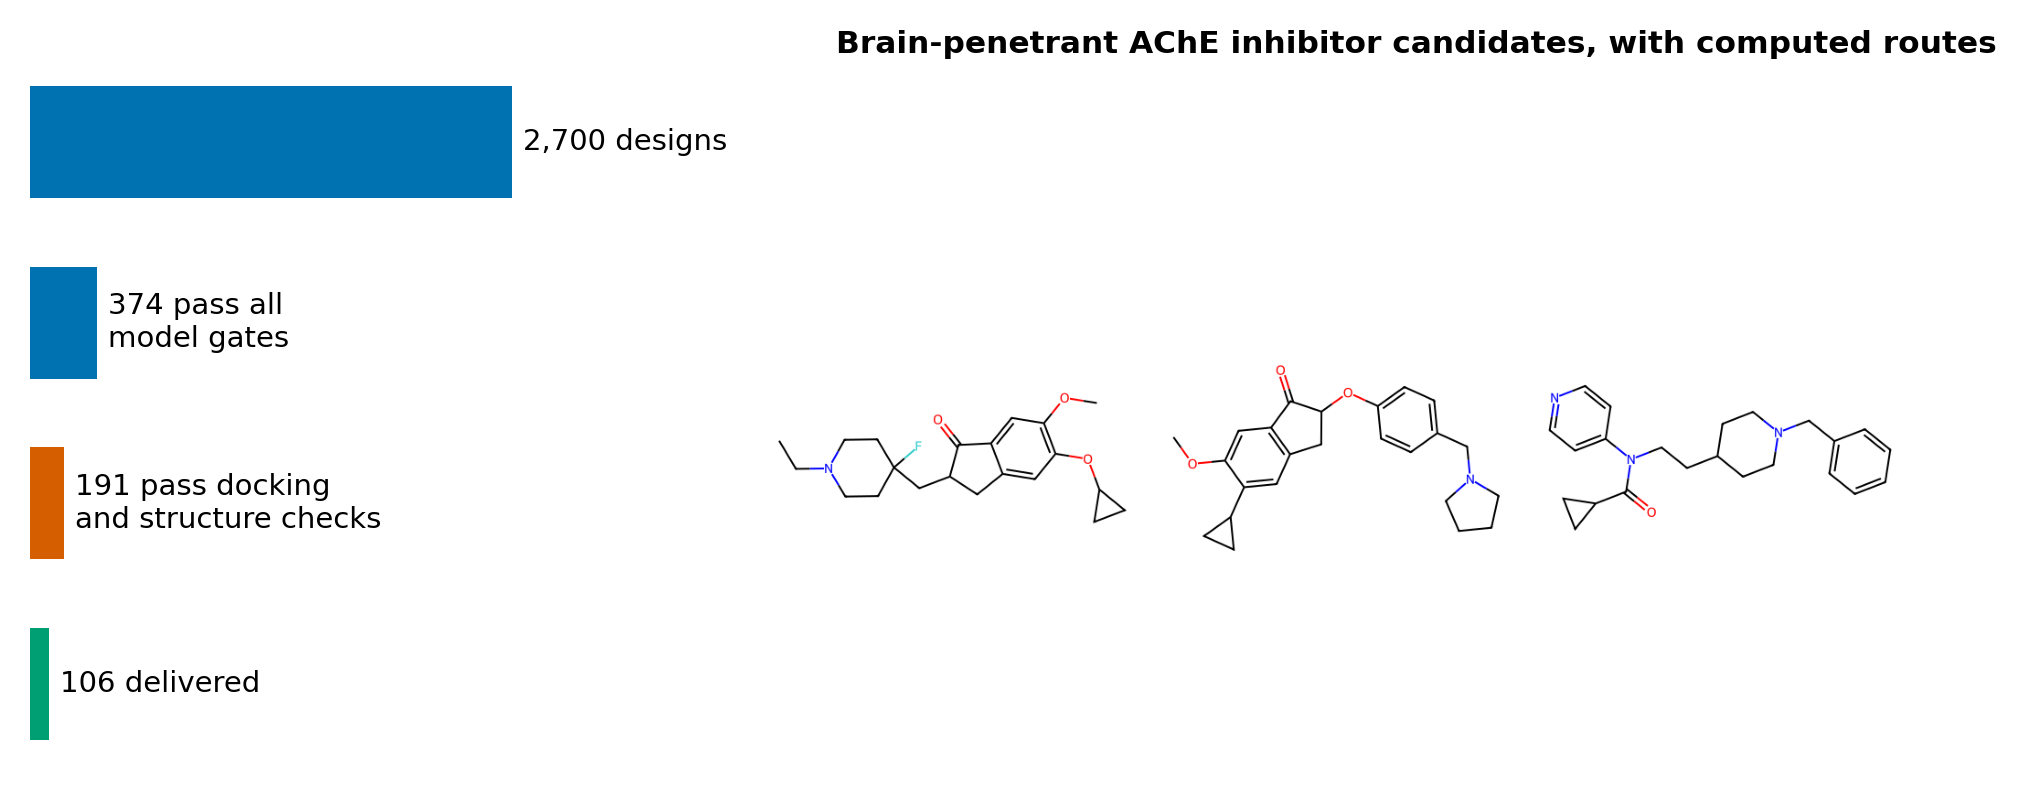
\includegraphics[width=13cm]{figures/TOC_graphic.png}
\newpage

\section{Introduction}
\label{sec:1}

Drugs for Alzheimer's disease must bind their target and reach the brain. The blood--brain barrier (BBB), a layer of tightly joined endothelial cells that carries efflux transporters such as P-glycoprotein (P-gp), keeps most circulating molecules out of the central nervous system.\cite{hu} Computational prioritization of such drugs therefore chains several models: an activity classifier, a permeability model, a brain-exposure estimate, a docking score and drug-likeness filters. A component of that chain is only as useful as its performance on molecules unlike its training data, and random data splits reward the recognition of close analogues,\cite{wallach} so scaffold-disjoint evaluation, in which no scaffold of the test set occurs in training, is the relevant test for a design campaign.\cite{murcko,tropsha}

Acetylcholinesterase (AChE, EC 3.1.1.7) is the validated target of donepezil, rivastigmine and galantamine, and the 2.35 \AA{} co-crystal structure of the human enzyme with donepezil (PDB ID 4EY7) resolves a ligand that spans the catalytic and the peripheral anionic site.\cite{sugimoto,pdb} Peripheral-site occupancy is also associated with inhibition of AChE-induced amyloid-$\beta$ aggregation.\cite{inest,ferrari} Thousands of measured inhibitors are available in ChEMBL,\cite{chembl} which makes AChE a suitable target for a data-driven design study, but a useful candidate must also be new, brain-penetrant and makeable. Computational papers on this target often stop at predicted potency; novelty and synthetic accessibility are checked less often and rarely by a computed route.

Here we describe a design cascade that turns published potent AChE inhibitors into a list of molecules that are, on every computed criterion we could apply, candidates to take to a chemist for synthesis planning. Candidates are generated by matched-molecular-pair (MMP) edits,\cite{hr,griffen} filtered by activity and permeability models trained on scaffold-disjoint partitions, by a validated logBB regression, by drug-likeness, toxicity and stability rules, by docking against 4EY7,\cite{vina,vina12} by protonation, tautomer and stereochemistry checks, by novelty searches in four independent sources, and finally by a computed retrosynthesis to purchasable starting materials.\cite{aizynth} The delivered set is every molecule that clears all gates, ordered by the margin with which it does so. We report what each component can and cannot support, because the margin of a molecule is only as meaningful as the models that define it, and we state plainly that no molecule has been synthesized or assayed.

%%BEGIN-CONTRIB
Figure~\ref{fig:workflow} gives an overview of the study. Our contributions are four. First, a gated design cascade whose components are each tested on held-out scaffolds against simple baselines, with the weak components named. Second, an anchoring of the design to measured AChE data: the edits are tested in real compound pairs, each molecule is tied to a measured parent, and the activity model is tested on compounds published later (Section~\ref{sec:anchor}). Third, a delivered set of 106 candidates, complete for the gates used, each with a computed route and a four-source novelty check, with a priority tier of 63 and a shortlist of 20. Fourth, falsifiable predictions for the first assay (Section~\ref{sec:discussion}), chosen so that the experiment discriminates between the structure-based and the ligand-based view of these molecules.

\begin{figure}[htbp]
\centering
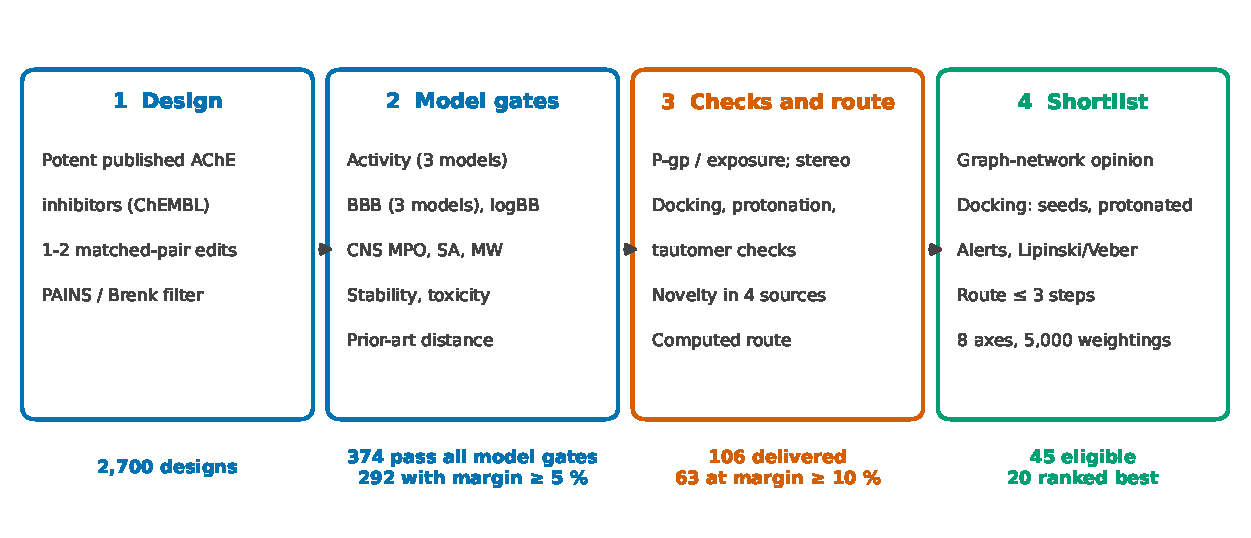
\includegraphics[width=\textwidth]{figures/Figure7.pdf}
\caption{Overview of the study. Counts are those of the delivered set; the gates are listed in Table~\ref{tab:1} and the shortlist ranking in Section~\ref{sec:best}.}
\label{fig:workflow}
\end{figure}

%%END-CONTRIB
\textit{Related work.} Machine-learning BBB models have been reported in this journal, for example an extra-trees model on B3DB with ROC-AUC 0.932 on a random partition\cite{liang} and a review of such models;\cite{nabi} LogBB\_Pred, published elsewhere, reports \textit{R}\textsuperscript{2} 0.61 for measured logBB.\cite{shaker} Most of these are evaluated on random partitions, which reward recognition of close analogues, so we report held-out-scaffold performance for every model we rely on. Structure-based screening for AChE has been reported in this journal with in vitro confirmation of 12 of 14 tested compounds,\cite{mokrani} and a graph generative adversarial network with reinforcement learning has been described for unconstrained generation.\cite{amodini} The present work constrains design to analogues of potent inhibitors, applies brain-penetration, novelty and synthesis criteria jointly, and stops short of experiment, which is the main respect in which it falls short of the AChE study cited. Docking benchmarks depend on how decoys are built,\cite{mysinger,chaput} and Vina pose accuracy is largely insensitive to box size and exhaustiveness,\cite{agarwal} so we tested both the pose and the score on our own system.

\section{Results and Discussion}
\label{sec:3}

\subsection{What the models behind the gates can support}
\label{sec:3.1}

Table~\ref{tab:2} gives the held-out performance of the components that define the gates. The activity model reaches ROC-AUC 0.900 on 1,289 held-out-scaffold compounds, ahead of nearest-neighbor similarity (0.871) and physicochemical descriptors (0.732), but on the least similar third of the test set it falls to 0.728 and is indistinguishable from nearest-neighbor lookup (0.720). It is therefore a reliable ranker near known chemistry, which is where every candidate lies (similarity to the nearest potent active 0.45--0.90, median 0.73), and it says little about unrelated chemotypes. The BBB classifier (AUC 0.802) beats the polar-surface-area baseline (0.721), and the scaffold-validated logBB regression (Spearman $\rho$ = 0.71) beats TPSA alone (0.65); both are used as the exposure evidence. Asking an independently trained second model to agree improved the precision of the activity selection (top-\textit{k} better in 16 of 20 scaffold partitions) but not that of the permeability selection (6 of 20), so the BBB gates rest on three models (two in-house and one independently trained on a different data set), and the second in-house model is not claimed to add independent information to the first.

%%BEGIN-SPLIT
The split protocol matters. On random 80/20 splits the BBB classifier and the activity model reach ROC-AUC 0.96 and 0.96; when whole scaffolds are assigned at random they reach 0.92 and 0.92; on the deterministic scaffold split used for every figure in this paper, in which the largest scaffold groups fill the training set and the test set holds the rarest scaffolds, they reach 0.80 and 0.90. For logBB the Spearman correlation falls from 0.79 under random cross-validation to 0.70 under scaffold-grouped cross-validation. Numbers from random splits, which dominate the BBB literature, therefore overstate what a design campaign can expect.

%%END-SPLIT
%%BEGIN-GNN
An independent graph neural network (edge-aware message passing on the molecular graph, five seeds, trained on the same training scaffolds and not tuned on the test partitions) reached ROC-AUC 0.813 (0.785--0.839) on the 1,289 held-out-scaffold compounds, against 0.900 for the random forest and 0.871 for nearest-neighbor lookup. Scored with it, the delivered molecules have a median activity probability of 0.92 (minimum 0.66); 106 of 106 reach 0.5 and 103 reach 0.7, and its probabilities correlate with those of the random forest at Spearman $\rho$ = 0.11. A second model family therefore supports the activity gate for the delivered set; the low rank correlation is expected, because both models place every candidate in a narrow band of high probability (random forest 0.74--0.94, graph network 0.66--1.00), within which their orderings carry little shared information.

%%END-GNN
\begin{table}[htbp]
\centering\small
\caption{Held-out performance of the components behind the gates (deterministic scaffold split unless stated).}
\label{tab:2}
\renewcommand{\arraystretch}{1.2}
\begin{tabular}{@{}>{\raggedright\arraybackslash}p{0.22\textwidth}>{\raggedright\arraybackslash}p{0.27\textwidth}>{\centering\arraybackslash}p{0.17\textwidth}>{\centering\arraybackslash}p{0.17\textwidth}@{}}
\toprule
\textbf{Component} & \textbf{Test} & \textbf{Result} & \textbf{Baseline} \\
\midrule
AChE activity & 1,289 held-out-scaffold compounds, AUC & 0.900 & NN 0.871 \\
AChE, least similar third & same, novelty tertile & 0.728 & NN 0.720 \\
BBB classifier & 1,165 compounds, AUC & 0.802 & $-$TPSA 0.721 \\
Martins BBB & 582 compounds, AUC & 0.929 & -- \\
logBB regression & 1,025, scaffold-grouped CV, $\rho$ & 0.71 & TPSA 0.65 \\
Docking pose & donepezil re-docked, 25 runs, RMSD & 0.83--0.92 \AA{} & 2.0 \AA{} \\
Docking score & 138 binders vs 526 matched decoys, AUC & 0.64 & properties 0.52 \\
P-gp term & BBB+ vs BBB$-$, permeable stratum, AUC & 0.52 & 0.60 required \\
hERG potency regression & 10,470 compounds, scaffold CV $\rho$; ten blockers vs ten non-blockers, AUC & 0.67; 1.00 & cisapride $>$ donepezil: not met \\
Matched-pair statistics & change in audit BBB probability & $-$0.100 & random $-$0.096 \\
\bottomrule
\end{tabular}
\end{table}

Three results limit how the gates should be read, and we state them because the delivered set rests on them. First, the docking score separated known binders from property-matched decoys only weakly (AUC 0.64, 0.59--0.69; Figure~\ref{fig:docking}), so the Vina gate is a plausibility filter on size and fit and is not evidence of potency; the pose of donepezil was reproduced within 0.9 \AA{} in all 25 re-docking runs, and pose coverage of the crystallographic footprint is the more informative structural criterion. Second, the P-gp term did not separate BBB-permeable from non-permeable compounds (AUC 0.52), and a composite exposure score that included it correlated with measured logBB at only $\rho$ = 0.24; the P-gp and exposure-surrogate gates are retained as conservative donepezil-anchored exclusions (they remove 26 candidates), but the logBB regression, not they, supplies the exposure evidence (Figure~\ref{fig:exposure}). Third, the matched-pair statistics selected edits no better than random edits, so the edit library is a source of chemically plausible analogues and the gates do the selecting. Two attempts to do better than Vina did not help: rescoring the same poses with the neural-network functions of GNINA gave AUC 0.47 to 0.70 against 0.72 for Vina on the first, molecular-weight-matched decoy set, and an independent co-folding check with Boltz-2 did not reach its enrichment bar (AUC 0.67, 0.54--0.81). No structural claim beyond docking is made.

%%BEGIN-DOCKSEEDS
Docking gates are reproducible for the delivered set: re-docking every molecule from two new random seeds (new starting conformer and new Vina seed) changed the Vina score by a median of 0.33 kcal mol\textsuperscript{$-$1} (95th percentile 0.94, maximum 1.36) across the three runs, the pose coverage of the donepezil footprint had a minimum of 0.54 over the runs (median 0.93), and 105 of 106 molecules (99\%) passed both docking gates in all three runs. The pre-specified criterion (at least 90 \% of molecules passing in all runs) was met.
%%END-DOCKSEEDS
\begin{figure}[htbp]
\centering
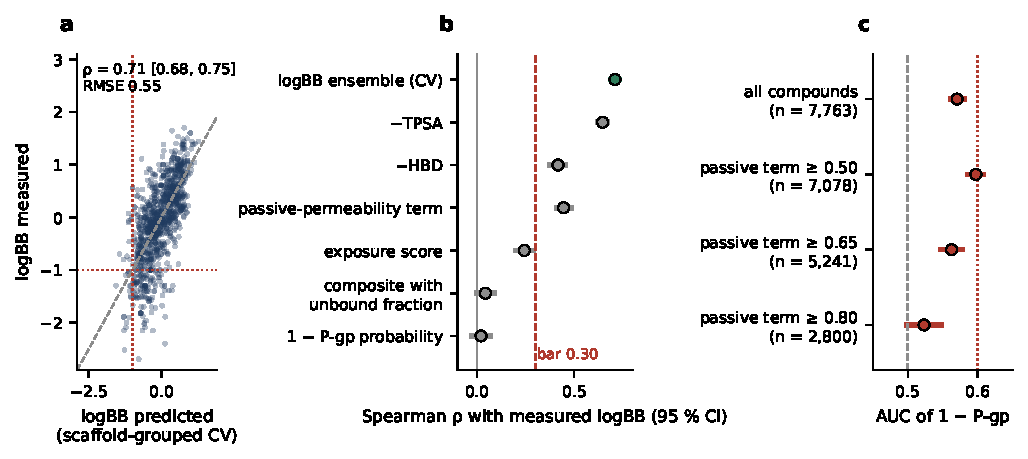
\includegraphics[width=\textwidth]{figures/Figure5.pdf}
\caption{Brain-exposure tests. (a) Out-of-fold logBB predictions of the scaffold-grouped cross-validated ensemble against measured values (\textit{n} = 1,025); dotted lines mark logBB = $-$1. (b) Spearman correlation with measured logBB (95 \% bootstrap intervals) for the exposure score, its two terms, two physicochemical descriptors and the cross-validated logBB ensemble; the dashed line is the pre-specified bar of 0.30. (c) ROC-AUC of one minus the P-gp probability for separating BBB+ from BBB$-$ compounds in B3DB, overall and within strata of increasing passive permeability; the dotted line is the pre-specified bar of 0.60.}
\label{fig:exposure}
\end{figure}

\begin{figure}[htbp]
\centering
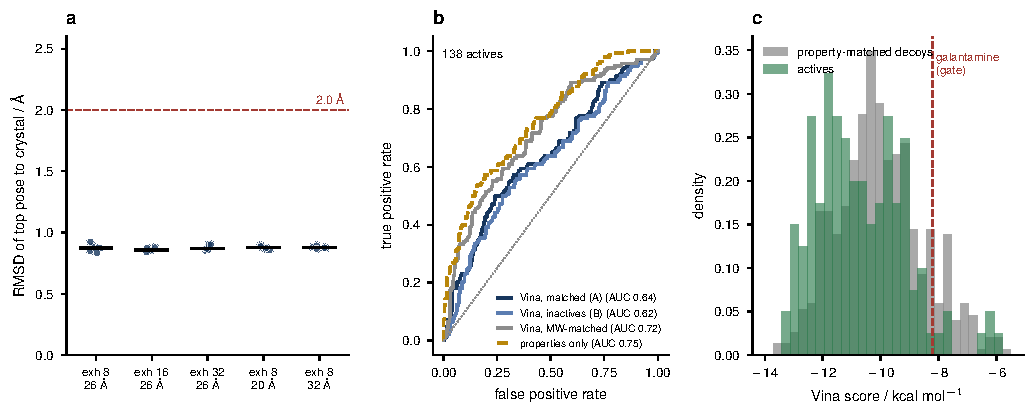
\includegraphics[width=\textwidth]{figures/Figure6.pdf}
\caption{Docking tests. (a) Heavy-atom RMSD of the top-ranked pose for donepezil re-docked into 4EY7 at three exhaustiveness values and three box sizes, five seeds each; the dashed line is the 2.0 \AA{} convention. (b) ROC curves of the Vina score on property-matched decoys (set A), on measured inactives (set B) and on a first, molecular-weight-matched decoy set, and of a classifier that sees only nine properties of that first set (no docking). (c) Distribution of Vina scores for the binders and the set-A decoys; the dashed line is galantamine's score.}
\label{fig:docking}
\end{figure}

\subsection{From 2,700 designs to 106 molecules}
\label{sec:3.2}

The 2,700 stored designs are themselves the survivors of the generation stage (Table~\ref{tab:gen}: 383,752 enumerated one- and two-edit analogues). Figure~\ref{fig:funnel} shows the funnel (the counts are also listed in the Supporting Information). The stored designs lose most of their number at the first four steps, where the activity and BBB models and the logBB gate act together; 374 designs pass every audited gate, and 292 of them clear 5 \% margin. The efflux and exposure gates, stereochemistry, docking, protonation and tautomer checks, novelty and retrosynthesis then reduce the 292 to the delivered 106. Of the 194 candidates that reached docking, one failed the docking gate and two the protonation check, and none was a tautomer of a known compound.

\begin{figure}[htbp]
\centering
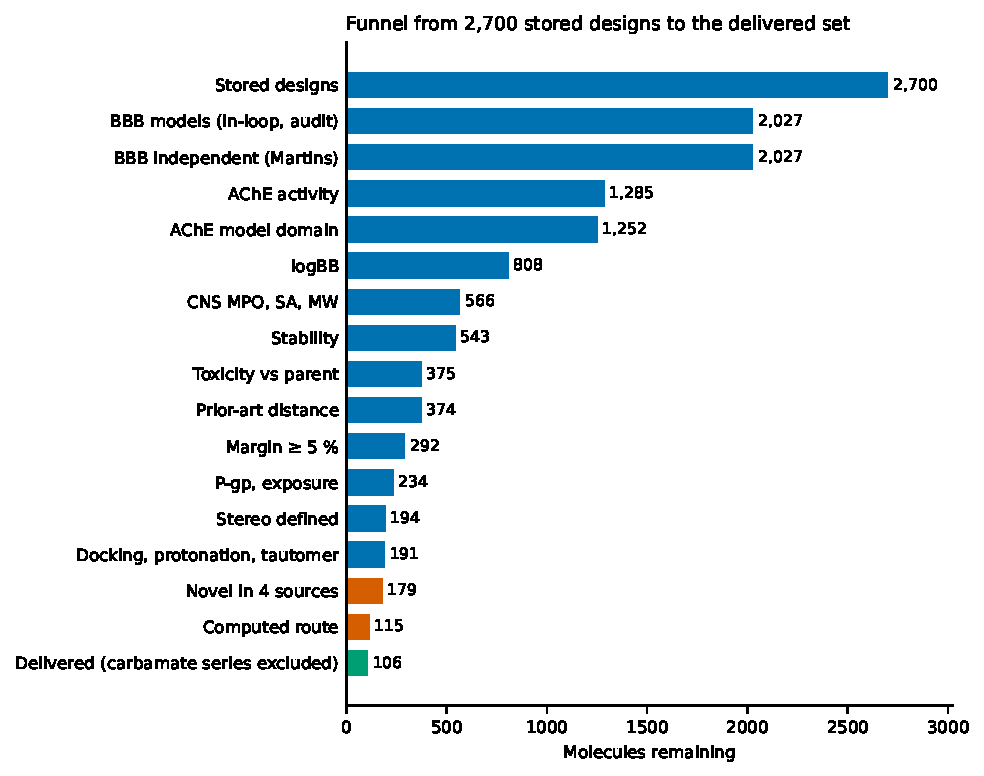
\includegraphics[width=0.9\textwidth]{figures/Figure1.pdf}
\caption{Funnel from the 2,700 stored designs to the delivered set. Blue, design-stage and structure-stage gates; orange, the novelty and synthesis gates; green, the delivered set.}
\label{fig:funnel}
\end{figure}


\subsection{The delivered set}
\label{sec:3.3}

The 106 molecules lie on 63 Bemis--Murcko scaffolds and come from 34 published parents; 39 carry one edit and 67 carry two. Their predicted properties are within the gates by construction, and the distributions show how far inside: the primary AChE probability has median 0.85 (minimum 0.74), both BBB models have median 0.88--0.89 (minimum 0.79), the independent Martins model 0.845 (minimum 0.75), and the predicted logBB has median 0.36 (minimum $-$0.21). The median molecule has MW 364, cLogP 3.9, TPSA 41 \AA{}\textsuperscript{2}, no hydrogen-bond donor and CNS MPO 4.3; the median Vina score is $-$10.85 kcal mol\textsuperscript{$-$1} and the median pose coverage of the donepezil footprint 0.96. The margin on the tightest audited gate is at least 5 \% for all molecules (median 11 \%, maximum 20.5 \%), and 63 molecules have at least 10 \%; these 63 form the priority tier (margin tier 1) and the other 43, with 5--10 \%, are tier 2. The tightest gate is a BBB model for 60 molecules and the logBB applicability domain for 26, which identifies where the set sits closest to the boundary of what these models support. Figure~\ref{fig:properties} shows the distributions and Table~\ref{tab:4} lists the twelve molecules with the largest margins (structures in Figure~\ref{fig:structures}).

\begin{figure}[htbp]
\centering
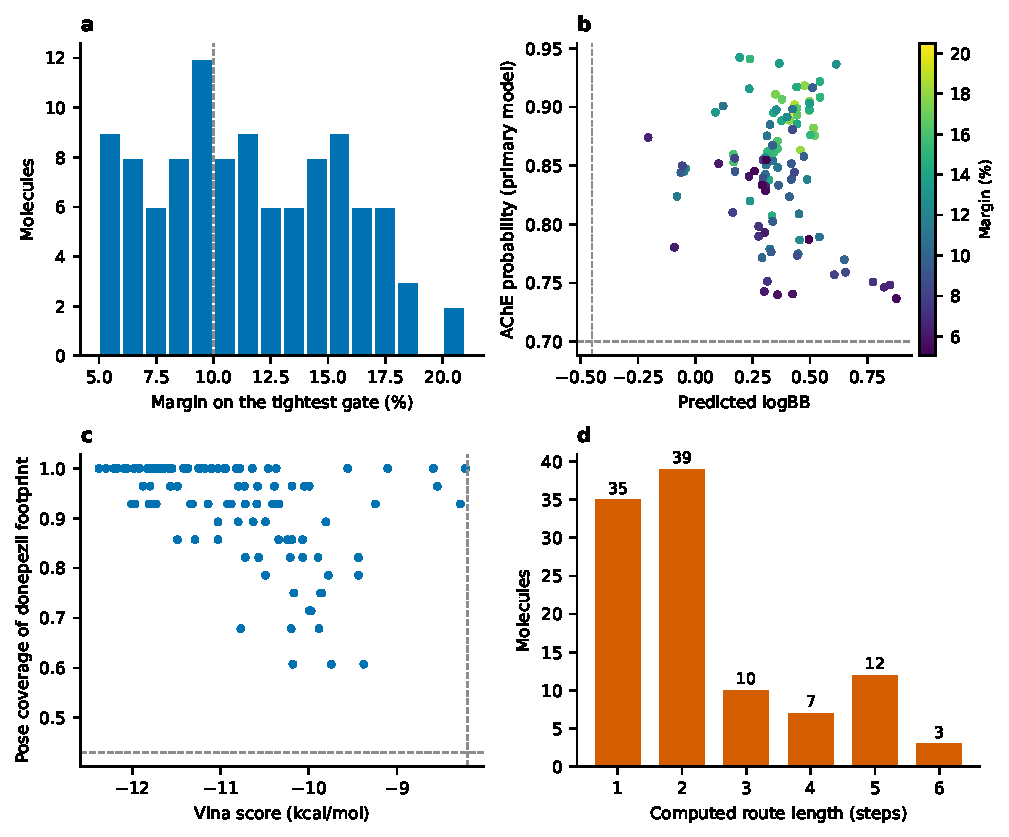
\includegraphics[width=\textwidth]{figures/Figure2.pdf}
\caption{Properties of the delivered set. (a) Margin on the tightest gate; the dashed line marks 10 \%. (b) Predicted logBB against the primary AChE probability, colored by margin; dashed lines are the gate thresholds. (c) Vina score against pose coverage of the donepezil footprint; dashed lines are the thresholds. (d) Length of the computed route.}
\label{fig:properties}
\end{figure}

\begin{table}[htbp]
\centering\footnotesize\setlength{\tabcolsep}{3pt}
\caption{The twelve delivered molecules with the largest margins (all 106 are in the Supporting Information). Edits: number of matched-pair transformations from the parent. AChE: primary probability. logBB: predicted. Vina in kcal mol\textsuperscript{$-$1} (a plausibility filter, not evidence of binding). Pose: coverage of the donepezil footprint. Margin: smallest slack (\%) on any audited gate. Steps: length of the longest linear sequence of the computed route (a convergent route contains more reactions in total; every reaction is listed in the dossier).}
\label{tab:4}
\renewcommand{\arraystretch}{1.2}
\begin{tabular}{@{}>{\raggedright\arraybackslash}p{0.04\textwidth}>{\centering\arraybackslash}p{0.43\textwidth}>{\centering\arraybackslash}p{0.06\textwidth}>{\centering\arraybackslash}p{0.07\textwidth}>{\centering\arraybackslash}p{0.07\textwidth}>{\centering\arraybackslash}p{0.07\textwidth}>{\centering\arraybackslash}p{0.06\textwidth}>{\centering\arraybackslash}p{0.07\textwidth}>{\centering\arraybackslash}p{0.06\textwidth}@{}}
\toprule
\textbf{No.} & \textbf{SMILES} & \textbf{Edits} & \textbf{AChE} & \textbf{logBB} & \textbf{Vina} & \textbf{Pose} & \textbf{Margin} & \textbf{Steps} \\
\midrule
% rows generated from results/SYNTHESIS_SET.csv (see top12_rows.tex)
1 & {\ttfamily\scriptsize\seqsplit{CCN1CCC(F)(CC2Cc3cc(OC4CC4)c(OC)cc3C2=O)CC1}} & 2 & 0.89 & 0.43 & $-$10.7 & 0.93 & 20 & 3 \\
2 & {\ttfamily\scriptsize\seqsplit{CCN1CCC(F)(CC2Cc3cc(OC)c(OC4CC4)cc3C2=O)CC1}} & 2 & 0.89 & 0.43 & $-$10.6 & 0.93 & 20 & 3 \\
3 & {\ttfamily\scriptsize\seqsplit{CCN1CCC(CC2Cc3cc(OC)c(OC4CC4)cc3C2=O)CC1}} & 2 & 0.90 & 0.43 & $-$9.8 & 0.89 & 19 & 1 \\
4 & {\ttfamily\scriptsize\seqsplit{CCN1CCC(CC2Cc3cc(OC4CC4)c(OC)cc3C2=O)CC1}} & 2 & 0.90 & 0.43 & $-$10.4 & 0.96 & 19 & 1 \\
5 & {\ttfamily\scriptsize\seqsplit{COc1cc2c(cc1C1CC1)CC(Oc1ccc(CN3CCCC3)cc1)C2=O}} & 2 & 0.86 & 0.46 & $-$11.2 & 1.00 & 18 & 5 \\
6 & {\ttfamily\scriptsize\seqsplit{O=C(C1CC1)N(CCC1CCN(Cc2ccccc2)CC1)c1ccncc1}} & 1 & 0.92 & 0.48 & $-$10.7 & 0.82 & 18 & 2 \\
7 & {\ttfamily\scriptsize\seqsplit{C=Cc1cc2c(cc1OC)C(=O)C(CC1CCN(Cc3ccccn3)CC1)C2}} & 2 & 0.89 & 0.41 & $-$12.1 & 1.00 & 18 & 2 \\
8 & {\ttfamily\scriptsize\seqsplit{COc1cc2c(cc1SC)CC(CC1CCN(Cc3ccccn3)CC1)C2=O}} & 1 & 0.90 & 0.50 & $-$11.8 & 1.00 & 18 & 2 \\
9 & {\ttfamily\scriptsize\seqsplit{COc1cc2c(cc1SC)C(=O)C(CC1CCN(Cc3ccccn3)CC1)C2}} & 1 & 0.90 & 0.50 & $-$11.6 & 1.00 & 18 & 2 \\
10 & {\ttfamily\scriptsize\seqsplit{COc1cc2c(cc1C)CC(CC1CCN(Cc3cccc(C)n3)CC1)C2=O}} & 1 & 0.88 & 0.52 & $-$12.4 & 1.00 & 17 & 4 \\
11 & {\ttfamily\scriptsize\seqsplit{O=C(CF)N(CCC1CCN(Cc2ccccc2)CC1)c1ccncc1}} & 2 & 0.91 & 0.35 & $-$9.9 & 0.75 & 17 & 2 \\
12 & {\ttfamily\scriptsize\seqsplit{O=C(c1ccncc1)N(CCC1CCN(Cc2ccccc2)CC1)C1CC1}} & 2 & 0.88 & 0.52 & $-$10.3 & 0.93 & 17 & 2 \\
\bottomrule
\end{tabular}
\end{table}

\begin{figure}[htbp]
\centering
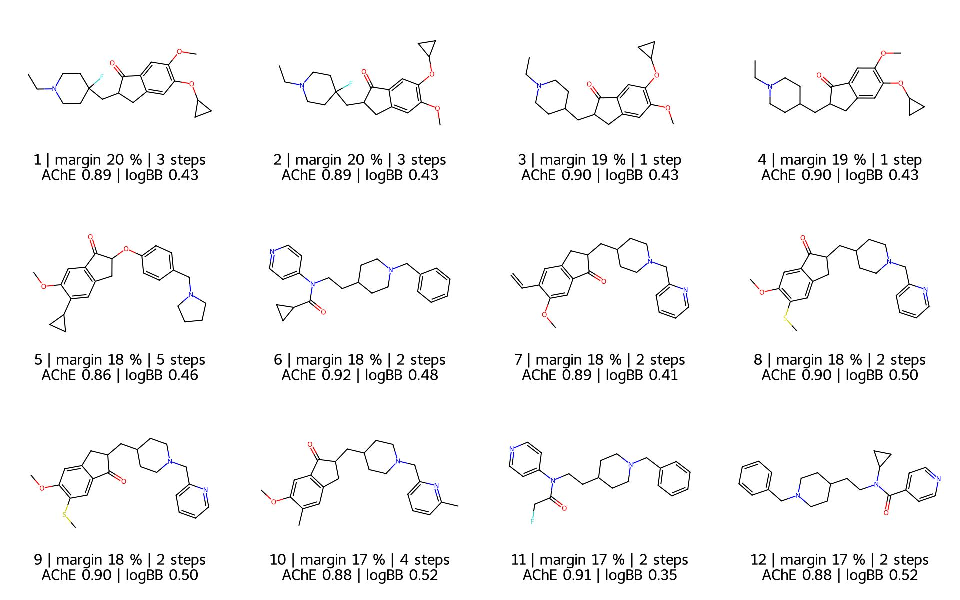
\includegraphics[width=\textwidth]{figures/Figure4.pdf}
\caption{Structures of the twelve delivered molecules with the largest margins, with primary AChE probability, predicted logBB, margin and the length of the computed route.}
\label{fig:structures}
\end{figure}


%%BEGIN-REFDRUGS
For orientation, \hyperref[tab:refdrugs]{Table~\ref{tab:refdrugs}} gives the established AChE drugs under the same models. Donepezil scores 0.99 on the activity model and tacrine 0.87, whereas the delivered set has a median of 0.85, so the candidates are not predicted to be more active than donepezil; their advantages in this study are predicted brain exposure, novelty and a computed route. The activity and BBB gates keep donepezil and tacrine and reject the others, which means that the cascade selects for donepezil-like and tacrine-like chemistry and is not a general AChE filter.

\begin{table}[htbp]
\centering\small
\caption{Established AChE drugs under the models and gates of this study (activity probability; BBB in-loop / audit / Martins; predicted logBB; CNS MPO; Vina in kcal mol\textsuperscript{$-$1}; pose coverage), and the median of the delivered set.}
\label{tab:refdrugs}
\begin{tabular}{@{}lcccccc@{}}
\toprule
\textbf{Compound} & \textbf{AChE} & \textbf{BBB} & \textbf{logBB} & \textbf{MPO} & \textbf{Vina} & \textbf{Pose} \\
\midrule
Donepezil & 0.99 & 0.99 / 0.95 / 0.85 & 0.75 & 4.1 & -11.8 & 1.00 \\
Galantamine & 0.50 & 0.47 / 0.52 / 0.90 & 0.31 & 5.8 & -8.2 & 0.43 \\
Rivastigmine & 0.28 & 0.24 / 0.38 / 0.84 & 0.82 & 5.3 & -7.8 & 0.82 \\
Tacrine & 0.87 & 0.90 / 0.76 / 0.88 & -0.30 & 5.4 & -8.8 & 0.57 \\
Huperzine A & 0.71 & 0.84 / 0.19 / 0.85 & -0.14 & 5.5 & -9.3 & 0.64 \\
\midrule
Delivered set (median) & 0.85 & 0.88 / 0.89 / 0.84 & 0.36 & 4.3 & -10.9 & 0.96 \\
\bottomrule
\end{tabular}
\end{table}
%%END-REFDRUGS
\textit{Novelty and its limits.} Every molecule is absent from PubChem (exact structure and same connectivity), ChEMBL (flexmatch) and SureChEMBL. Twelve candidates that passed everything before the novelty search were removed because PubChem, ChEMBL or SureChEMBL found them, some in more than one source. The nearest potent ChEMBL active of each molecule has median Tanimoto similarity 0.73 (0.45--0.90), and 38 molecules (12 of the 63 scaffolds) carry a Bemis--Murcko scaffold that already occurs among ChEMBL AChE compounds. The molecules are therefore close analogues within known donepezil-like, tacrine-like and related series and not new chemotypes (Figure~\ref{fig:space}). A negative database search shows that the exact structure has not been indexed; it does not exclude disclosure within the scope of a patent claim. We found direct evidence of that gap for one series. The eseroline phenylcarbamates, to which nine otherwise eligible candidates belong (including the one with the largest margin before this exclusion, a 2-fluorophenyl analogue of phenserine), derive from parents that are the subject of a patent family on substituted phenserines\cite{greigpatent} (now expired) and of systematic work on the aryl ring of the carbamate.\cite{yu2001} Such disclosures are prior art whose scope a structure query does not capture, so these nine were excluded for novelty and the set is reported without them. The same caution applies in principle to the remaining series, whose parents are also published drugs and drug candidates: a database miss is not a novelty opinion, and novelty and freedom to operate must be assessed by a patent attorney; neither is asserted here.

\begin{figure}[htbp]
\centering
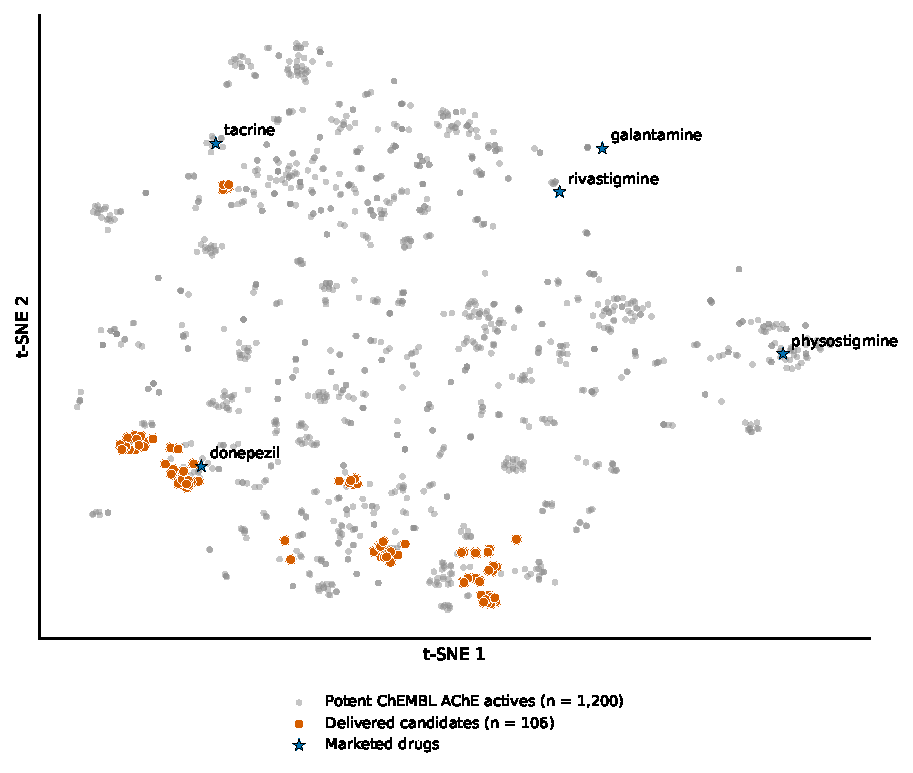
\includegraphics[width=0.8\textwidth]{figures/Figure3.pdf}
\caption{Chemical space of the delivered candidates. t-SNE embedding (Jaccard distance on ECFP4) of 1,200 potent ChEMBL AChE actives, the delivered candidates and five marketed drugs.}
\label{fig:space}
\end{figure}

\textit{Synthesis.} All 106 molecules have a computed route whose leaves are purchasable: 35 in one step, 39 in two, 10 in three, 7 in four, 12 in five and 3 in six, with a median route score of 0.994 (minimum 0.956). The routes stem from literature reaction templates and are hypotheses for a chemist to review. No computed route passes through the parent: the tool builds each molecule directly from purchasable building blocks. The parent is listed by suppliers for 27 of the 106 molecules and not for 79, so parent availability does not limit the routes, although a chemist may prefer a late-stage modification of a catalogued parent where one exists. Stereochemistry is fully specified: 65 molecules carry defined stereocenters from their parents or by design, and 41 are specified as racemates because every undefined center lies $\alpha$ to a carbonyl and epimerizes.

%%BEGIN-BENCH
As a reference for these rates, the same first-pass search (200 iterations, 120 s) found a route for 52 of 80 (65 \%) randomly chosen potent ChEMBL AChE actives and for 3 of 6 established AChE drugs (donepezil (route), tacrine (route), galantamine (no route), rivastigmine (route), huperzine A (no route), physostigmine (no route)), against 95 of 179 (53 \%) of the novelty-clear candidates; the second, deeper pass added 20 candidates. The difference is not significant (Fisher exact $p$ = 0.08), so the candidates are not detectably harder to route than known inhibitors. The tool also misses some established drugs, so ``no route found'' should not be read as ``not makeable''.

%%END-BENCH
\textit{Structural plausibility.} Most molecules belong to the donepezil family: 77 of the 106 carry an N-alkylpiperidine, 41 an indanone and 36 an N-benzylpiperidine or N-benzylpyrrolidine, and six are tacrine-like. The four molecules with the largest margins, and a fifth at rank 46, are N-ethyl indanone-piperidines in which donepezil's benzyl ring is replaced by an ethyl group. In our docked poses these molecules keep the peripheral-site stacking of the indanone ring but no longer have an aromatic ring to stack on Trp86, and their docking scores do not register that loss; they rank high because the smaller, less lipophilic structure raises the predicted logBB and the BBB margins. Three molecules of the delivered set (ranks 1, 2 and 4) were tested earlier in 2 ns of explicit-solvent molecular dynamics with one replica each. Two kept their pose (second-half RMSD 2.5 and 0.8 \AA{}) and one drifted (3.6 \AA{}, above the 3.0 \AA{} criterion). This is a screen and not converged sampling, and the other 103 molecules were not simulated.

%%BEGIN-BEST-RESULTS
\subsection{A shortlist of twenty molecules for first synthesis}
\label{sec:shortlist}

To choose where to start, the 63 priority-tier molecules were put through every remaining computational check and ranked (Section~\ref{sec:best}). The independent graph network removed 2, the docking gates in all three seed runs and after re-docking with the protonated amine removed 1, structural alerts removed 4 (none of the 106 has a PAINS or Brenk alert; 4 carry a NIH alert, among them a monofluoroacetamide and three alpha-halo heteroatom groups), a route longer than three steps removed 11, and no molecule violated the Lipinski or Veber criteria. The 45 that remained were ranked on eight evidence axes under 5,000 random weightings, and the twenty with the best median rank, with at most two per scaffold and four per parent, are listed in \hyperref[tab:best]{Table~\ref{tab:best}}. They lie on 16 scaffolds from 10 parents, have a median margin of 14.7 \% and a median graph-network probability of 0.96, and a median worst-case Vina score of $-$11.3 kcal mol\textsuperscript{$-$1}; 10 with a one-step route, 6 with two steps, 4 with three steps, and 6 stack on both Trp86 and Trp286 with the protonated amine, as donepezil does. The order inside the list is not firm: the median width of the 5th--95th percentile rank interval is 23 positions, so the list is robust as a group and its individual order is not. All twenty still carry the open issues stated elsewhere in this paper, above all that hERG block and potency are unmeasured, and the list is a proposal for a first synthesis batch, not a finding.

\begin{table}[htbp]
\centering\footnotesize\setlength{\tabcolsep}{3pt}
\caption{The shortlist of twenty molecules for first synthesis, in order of median rank under 5,000 random weightings of eight evidence axes. Margin: smallest slack on any audited gate (\%). GNN: probability from the independent graph network. Vina: worst of four docking runs (kcal mol\textsuperscript{$-$1}). Steps: longest linear sequence of the computed route. Contacts: Trp86 stacking, Trp286 stacking and cation--$\pi$ contact in the protonated re-docking (0--3).}
\label{tab:best}
\renewcommand{\arraystretch}{1.2}
\begin{tabular}{@{}>{\raggedright\arraybackslash}p{0.05\textwidth}>{\centering\arraybackslash}p{0.52\textwidth}>{\centering\arraybackslash}p{0.09\textwidth}>{\centering\arraybackslash}p{0.07\textwidth}>{\centering\arraybackslash}p{0.08\textwidth}>{\centering\arraybackslash}p{0.07\textwidth}>{\centering\arraybackslash}p{0.09\textwidth}@{}}
\toprule
\textbf{No.} & \textbf{SMILES} & \textbf{Margin} & \textbf{GNN} & \textbf{Vina} & \textbf{Steps} & \textbf{Contacts} \\
\midrule
1 & {\ttfamily\scriptsize\seqsplit{COc1cc2c(cc1SC)CC(CC1CCN(Cc3ccccn3)CC1)C2=O}} & 17.5 & 0.94 & $-$11.5 & 2 & 3 \\
2 & {\ttfamily\scriptsize\seqsplit{COc1cc2c(cc1SC)C(=O)C(CC1CCN(Cc3ccccn3)CC1)C2}} & 17.5 & 0.94 & $-$11.6 & 2 & 3 \\
3 & {\ttfamily\scriptsize\seqsplit{O=C(CCC1CCN(CC2CC2)CC1)c1cc2c3c(c1)CC(=O)N3CCC2}} & 14.3 & 0.99 & $-$11.7 & 1 & 2 \\
4 & {\ttfamily\scriptsize\seqsplit{COc1cc2c(cc1OC1CC1)C(=O)C(CC1CCN(Cc3ccccn3)CC1)C2}} & 16.8 & 0.92 & $-$11.2 & 2 & 3 \\
5 & {\ttfamily\scriptsize\seqsplit{COc1cc2c(cc1OC)C(=O)C(CC1CCN(Cc3ccc(CO)cc3)CC1)C2}} & 13.7 & 0.93 & $-$11.7 & 2 & 3 \\
6 & {\ttfamily\scriptsize\seqsplit{O=C(CCC1CCN(CCC2CC2)CC1)c1cc2c3c(c1)CCC(=O)N3CCC2}} & 12.6 & 0.99 & $-$11.6 & 1 & 2 \\
7 & {\ttfamily\scriptsize\seqsplit{O=C(CCC1CCN(CC2CC2)CC1)c1cc2c3c(c1)CCC(=O)N3CCC2}} & 12.7 & 0.99 & $-$11.6 & 1 & 2 \\
8 & {\ttfamily\scriptsize\seqsplit{COc1cc2c(cc1OC1CC1)CC(CC1CCN(Cc3ccccn3)CC1)C2=O}} & 16.8 & 0.92 & $-$11.0 & 2 & 3 \\
9 & {\ttfamily\scriptsize\seqsplit{CCN1CCC(CC2Cc3cc(OC4CC4)c(OC)cc3C2=O)CC1}} & 18.7 & 0.96 & $-$10.2 & 1 & 2 \\
10 & {\ttfamily\scriptsize\seqsplit{CCN1CCC(F)(CC2Cc3cc(OC)c(OC4CC4)cc3C2=O)CC1}} & 20.5 & 0.96 & $-$10.0 & 3 & 2 \\
11 & {\ttfamily\scriptsize\seqsplit{COc1cc2c(cc1C)C(=O)C(Oc1ccc(CN3CCCC3)cc1)C2}} & 15.8 & 0.95 & $-$11.5 & 3 & 2 \\
12 & {\ttfamily\scriptsize\seqsplit{CCN1CCC(CCC(=O)c2cc3c4c(c2)CC(=O)N4CCC3)CC1}} & 14.3 & 0.99 & $-$11.1 & 1 & 2 \\
13 & {\ttfamily\scriptsize\seqsplit{CCN1CCC(CC2Cc3cc(OC)c(OC4CC4)cc3C2=O)CC1}} & 18.7 & 0.96 & $-$9.8 & 1 & 2 \\
14 & {\ttfamily\scriptsize\seqsplit{O=C(CCC1CCN(CCC2CC2)CC1)c1cc2c3c(c1)CC(=O)N3CCC2}} & 14.3 & 1.00 & $-$11.2 & 1 & 2 \\
15 & {\ttfamily\scriptsize\seqsplit{CCN1CCC(F)(CC2Cc3cc(OC4CC4)c(OC)cc3C2=O)CC1}} & 20.5 & 0.96 & $-$9.7 & 3 & 2 \\
16 & {\ttfamily\scriptsize\seqsplit{O=C(CCC1CCN(Cc2ccccc2F)CC1)c1ccc2c(c1)OCCO2}} & 13.6 & 0.85 & $-$12.1 & 2 & 3 \\
17 & {\ttfamily\scriptsize\seqsplit{CCCN1CCC(CCC(=O)c2cc3c4c(c2)CC(=O)N4CCC3)CC1}} & 11.1 & 0.99 & $-$11.1 & 1 & 2 \\
18 & {\ttfamily\scriptsize\seqsplit{COc1cc2c(cc1C)C(=O)C(Oc1cccc(CN3CCCCC3)c1)C2}} & 15.2 & 0.96 & $-$11.4 & 3 & 2 \\
19 & {\ttfamily\scriptsize\seqsplit{CCCN1CCC(CCNC(=O)c2ccc3cc(OC)ccc3c2)CC1}} & 10.7 & 0.96 & $-$10.7 & 1 & 2 \\
20 & {\ttfamily\scriptsize\seqsplit{CCN1CCC(CCC(=O)c2cc3c4c(c2)CCC(=O)N4CCC3)CC1}} & 12.6 & 0.99 & $-$11.3 & 1 & 2 \\
\bottomrule
\end{tabular}
\end{table}

%%END-BEST-RESULTS
%%BEGIN-ANCHOR-RESULTS
\subsection{Anchoring the delivered set to measured AChE data}
\label{sec:anchor}

Review of the design raised two questions: do the edits, which were mined from brain-penetration data, keep AChE potency, and how close is each molecule to something measured? We answered them with the measured AChE data of ChEMBL (5,814 compounds).

Edits in real pairs. For the 22 transformations of the delivered set we found every pair of measured AChE compounds that differ by exactly that exchange, in the design direction and from the same publication (Table~\ref{tab:edits}); 17 of the 22 transformations have at least three such pairs. Over 961 pairs (472 publications), 64.5 \% of the pairs changed pChEMBL by 0.5 log units or less (95 \% interval over publications 59.6--70.0 \%) and 3.7 \% lost more than one log unit (2.5--5.3 \%); for all other exchanges between measured compounds (196,669 pairs) the shares were 51.6 \% (47.8--55.8 \%) and 11.8 \% (10.0--13.5 \%). The edits used are therefore conservative substitutions that, on average, preserve potency; this is expected of small exchanges such as methyl for cyclopropyl or chloro for fluoro, and is not evidence that any single edit preserves it. The exceptions are visible in Table~\ref{tab:edits}: removing a phenyl ring (14 molecules) lost more than one log unit in 12 \% of its 92 pairs, as often as arbitrary exchanges, and methyl to cyclopropylmethyl (11 molecules) rests on 4 pairs only.

Parents and what to expect. 104 of the 106 molecules have a measured parent (median pChEMBL 7.16, about 69 nM; range 6.57 to 8.44) and none is itself a measured compound; the most similar measured compound has a median ECFP4 similarity of 0.75 (Table~\ref{tab:anchor} lists the shortlist). We asked whether the edit-specific change seen in real pairs can refine that expectation: predicting each pair's change from the median change of the same exchange in other publications was no better than predicting no change (mean absolute error 0.482 against 0.475 log units; Spearman correlation 0.058 between predicted and observed change; 954 pairs of 17 exchanges). The best expectation for a molecule is therefore the potency of its parent, with a typical change of about half a log unit in either direction, and a loss of more than one log unit in about one pair in twenty-five.

Time-split validation inside the applicability domain. The activity gate admits only molecules whose similarity to the nearest potent training active is at least 0.417 (Section~\ref{sec:2.2}). Repeating the time-split test for the later compounds that satisfy that condition (41, 46 and 48 \% of later compounds at the three cutoffs), the activity design reached ROC-AUC 0.79, 0.81 and 0.85 against 0.67, 0.68 and 0.72 for nearest-neighbour similarity and 0.64, 0.69 and 0.73 for the descriptor model, with non-overlapping intervals; outside the domain it reached 0.60, 0.63 and 0.64. The pre-specified bar (2015 cutoff, in domain, above both baselines and above 0.65) was met. We state that this analysis was added after the earlier test failed in the least-similar third, motivated by the domain gate the design already enforced, and we report both.

Calibration and abstention. For later compounds the model's probabilities were reasonably calibrated in the most similar third (expected calibration error 0.04) and poorly calibrated in the least similar (0.14); conformal prediction sets aimed at 90 \% coverage covered 65 \% of all later compounds and 44 \% of the least similar third, so the usual coverage guarantee does not hold under this temporal shift. Abstaining below a nearest-neighbour similarity of 0.343 raised accuracy at 0.5 from 0.722 to 0.798 while keeping 67 \% of compounds, in line with the domain gate.

Blind re-discovery. Using only compounds reported up to a cutoff year, we applied the design stage's edits to the potent parents and asked how many compounds reported later were reproduced exactly and how close the generated analogues came to later potent compounds: at the 2015 cutoff the design-stage edits generated 325,244 analogues from 1,247 earlier potent parents and reproduced 7 of the 2,784 later compounds exactly (5 of the 593 later potent compounds), against 5 to 8 (2 to 3 potent) for 3 random draws of unused edits; the share of later potent compounds with a generated analogue at ECFP4 similarity of at least 0.8 was 2.9 % for the design-stage edits and 2.0 to 2.9 % for the random draws (mean highest similarity 0.48 against 0.47 to 0.47); at the 2018 cutoff the design-stage edits generated 345,702 analogues from 1,531 earlier potent parents and reproduced 6 of the 1,819 later compounds exactly (3 of the 393 later potent compounds), against 4 to 4 (1 to 3 potent) for 3 random draws of unused edits; the share of later potent compounds with a generated analogue at ECFP4 similarity of at least 0.8 was 2.5 % for the design-stage edits and 1.5 to 2.3 % for the random draws (mean highest similarity 0.49 against 0.47 to 0.48); at the 2012 cutoff (exact matches only) the design-stage edits reproduced 5 later compounds (4 potent) against 3 to 8 (2 to 3 potent) for 2 random draws. Exact re-discovery is rare and the counts are too small to separate the edit sets, and the near-recovery measure shows at most a small difference (the design-stage edits are within the range of the random draws at 2015 and slightly above it at 2018): the edit library has not been shown to find future compounds clearly better than other edits, which agrees with the matched-pair statistics test of Table~\ref{tab:1}. The value of the cascade therefore lies in its gates and its anchoring to measured parents and not in the edit selection.

\begin{figure}[htbp]
\centering
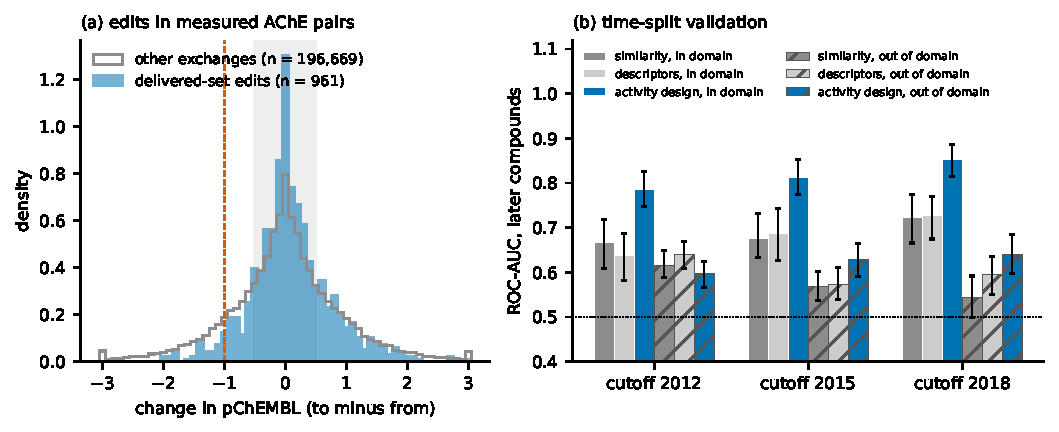
\includegraphics[width=\textwidth]{figures/Figure8.pdf}
\caption{Anchoring to measured AChE data. (a) Change in pChEMBL for same-publication pairs of measured compounds that differ by one of the 22 delivered-set exchanges (blue) and for all other exchanges (grey); the shaded band is 0.5 log units either side of zero and the dashed line a loss of one log unit. (b) Time-split ROC-AUC (95 \% bootstrap interval) of the activity design and the two baselines for later-published compounds inside and outside the applicability domain of the activity gate (similarity to the nearest training active of at least 0.417).}
\label{fig:anchor}
\end{figure}

\begin{table}[htbp]
\centering\small
\caption{The twelve most used edits of the delivered set in real AChE compound pairs. Molecules: delivered molecules carrying the edit (as its second edit for two-edit molecules). Pairs: pairs of measured compounds from the same publication that differ by exactly this exchange in the design direction; Median: median change in pChEMBL (to minus from); Within: share of pairs changing by 0.5 log units or less; Lose: share losing more than one log unit. Me, methyl; Et, ethyl; Pr, propyl; Ph, phenyl; cPr, cyclopropyl; OAc, acetoxy; HEP, hydroxyethylpiperazinyl.}
\label{tab:edits}
\resizebox{\textwidth}{!}{%
\begin{tabular}{lcccccc}
\toprule
Edit & Molecules & Pairs & Publications & Median & Within & Lose \\
\midrule
Me$\to$cPr & 22 & 8 & 5 & +0.09 & 88 \% & 0 \% \\
Ph$\to$Me & 14 & 92 & 49 & +0.11 & 47 \% & 12 \% \\
Me$\to$CH2cPr & 11 & 4 & 4 & +0.91 & 0 \% & 0 \% \\
OMe$\to$Me & 11 & 106 & 49 & -0.03 & 67 \% & 3 \% \\
Et$\to$Pr & 8 & 80 & 21 & -0.10 & 72 \% & 4 \% \\
OMe$\to$SMe & 7 & 4 & 2 & -0.29 & 75 \% & 0 \% \\
OMe$\to$Cl & 6 & 98 & 48 & +0.01 & 68 \% & 4 \% \\
Cl$\to$F & 5 & 109 & 50 & +0.00 & 68 \% & 2 \% \\
CH2Cl$\to$CH2OH & 4 & 2 & 2 & +0.64 & 0 \% & 0 \% \\
Et$\to$Me & 2 & 244 & 73 & +0.08 & 66 \% & 2 \% \\
Me$\to$Cl & 2 & 96 & 43 & +0.17 & 59 \% & 2 \% \\
cPr$\to$Et & 2 & 6 & 3 & -0.04 & 67 \% & 33 \% \\
\bottomrule
\end{tabular}}
\end{table}

\begin{table}[htbp]
\centering\small
\caption{The shortlist anchored to measured AChE data. Parent: measured pChEMBL of the potent published parent. Edits: the one or two matched-pair edits. Nearest measured: ECFP4 similarity and pChEMBL of the most similar measured AChE compound. P(active): activity-model probability.}
\label{tab:anchor}
\resizebox{\textwidth}{!}{%
\begin{tabular}{rcllc}
\toprule
Rank & Parent & Edits & Nearest measured & P(active) \\
\midrule
1 & 6.8 & OMe$\to$SMe & 0.83 / 6.8 & 0.90 \\
2 & 6.8 & OMe$\to$SMe & 0.83 / 6.8 & 0.90 \\
3 & 8.4 & Ph$\to$Me, Me$\to$cPr & 0.73 / 8.4 & 0.90 \\
4 & 6.8 & Me$\to$cPr & 0.90 / 6.8 & 0.91 \\
5 & 6.9 & Me$\to$CH2Cl, CH2Cl$\to$CH2OH & 0.83 / 6.9 & 0.94 \\
6 & 7.8 & Ph$\to$Me, Me$\to$CH2cPr & 0.74 / 7.8 & 0.89 \\
7 & 7.8 & Ph$\to$Me, Me$\to$cPr & 0.74 / 7.8 & 0.90 \\
8 & 6.8 & Me$\to$cPr & 0.90 / 6.8 & 0.91 \\
9 & 7.6 & Me$\to$cPr, Ph$\to$Me & 0.67 / 8.1 & 0.90 \\
10 & -- & Me$\to$cPr, Ph$\to$Me & 0.48 / 8.1 & 0.89 \\
11 & 6.9 & OMe$\to$Me & 0.86 / 6.9 & 0.86 \\
12 & 8.4 & Ph$\to$Me & 0.73 / 8.4 & 0.84 \\
13 & 7.6 & Me$\to$cPr, Ph$\to$Me & 0.67 / 8.1 & 0.90 \\
14 & 8.4 & Ph$\to$Me, Me$\to$CH2cPr & 0.73 / 8.4 & 0.89 \\
15 & -- & Me$\to$cPr, Ph$\to$Me & 0.48 / 8.1 & 0.89 \\
16 & 7.5 & Ph$\to$2-F-Ph & 0.75 / 7.5 & 0.94 \\
17 & 8.4 & Ph$\to$Me, Et$\to$Pr & 0.71 / 8.4 & 0.88 \\
18 & 6.6 & OMe$\to$Me & 0.87 / 6.6 & 0.86 \\
19 & 6.7 & Ph$\to$Me, Et$\to$Pr & 0.74 / 6.7 & 0.77 \\
20 & 7.8 & Ph$\to$Me & 0.74 / 7.8 & 0.86 \\
\bottomrule
\end{tabular}}
\end{table}

%%END-ANCHOR-RESULTS
\subsection{Safety and selectivity flags}
\label{sec:3.4}

No molecule has a toxicity probability more than 0.10 worse than that of its parent, but the absolute values are not reassuring. The predicted hERG probability has median 0.85 (maximum 0.93), as it does for the donepezil-like parents, and the hERG classifier could not rank cisapride, a far more potent blocker, above donepezil when we tested it, so the value cannot be used to separate candidates; hERG liability must be measured and is the most likely reason for a candidate to fail. We therefore tried a second model, a regression on the measured potencies of 10,470 ChEMBL compounds, with its pass criteria fixed beforehand. It ranked unseen scaffolds well (scaffold-grouped cross-validated Spearman $\rho$ = 0.67, AUC 0.82 for IC\textsubscript{50} $\leq$ 10 \textmu{}M) and separated ten potent blockers from ten drugs without meaningful hERG block perfectly (AUC 1.00, panel structures held out of training), but it failed the third criterion, that cisapride be predicted more potent than donepezil (5.37 against 5.69 in pChEMBL units), because its predictions are compressed toward the mean: the delivered molecules span only 5.15--6.06 and 55 of 106 are predicted slightly weaker than their parent. By the rule that all three criteria must hold, it was not used to label the molecules, and the statement stands that hERG block cannot yet be ranked computationally for this set. Ames and DILI probabilities have median 0.49 and 0.45. For butyrylcholinesterase, 104 molecules have a higher predicted AChE than BChE probability, and 30 have a predicted BChE probability of at least 0.5, which is not a defect for Alzheimer's disease but should be known when interpreting an assay. The BCRP similarity flag, which failed its own calibration, flags one molecule (rank 94) and is not evidence of absence of BCRP efflux for the others. P-gp and BCRP efflux were not measured.

%%BEGIN-DISCUSSION
\subsection{Discussion and falsifiable predictions}
\label{sec:discussion}

This study does not claim that the delivered molecules are better inhibitors than donepezil; the activity models score donepezil higher than the delivered set, and no potency has been measured. What it offers is a worked, audited route from published inhibitors to makeable, novel-by-search, brain-penetrant candidates, in which every gate has a stated validity and the weak ones are named. The molecules sit close to known donepezil-like series, so the realistic expectation is activity of the same kind as that series and hERG liability like its parents; novelty would lie in the exact structures and in the pathway, and the chance of a clinical advantage is small.

The first assay should be designed to test something. The activity models and the structure-based view disagree about one feature. In the protonated re-docking, 44 of the 106 molecules place an aromatic ring on Trp86, as donepezil's benzyl ring does (37 of them carry a benzyl-type N-CH\textsubscript{2}-aryl group), and 62 do not (37 of these have only small alkyl groups on the basic nitrogen and 25 have a benzyl-type group that does not reach Trp86 in the top pose). The random forest scores the stackers slightly higher (mean probability 0.87 against 0.84) but the graph network scores them lower (0.86 against 0.92), so ligand-based models do not register the difference. Structure-based reasoning predicts that molecules that keep the Trp86 interaction are markedly more potent than those that lose it. We state that as a prediction: in an Ellman assay with donepezil on the same plate, the stackers should have clearly lower IC\textsubscript{50} values than the non-stackers within each chemical series, and if they do not, the structure-based reading of this pocket is wrong for these compounds. Two further predictions are that the first-pass computed routes succeed in the laboratory for most of the one- and two-step molecules, and that every active molecule shows hERG block at micromolar concentrations, as the parents do; a molecule that is both active and free of hERG block would be the finding worth following.

%%END-DISCUSSION
%%BEGIN-TIMEMD-RESULTS
\subsection{Temporal validation and pose stability of the shortlist}
\label{sec:timeresults}

Time-split validation (Table~\ref{tab:time}). Trained only on compounds reported up to a cutoff year, the activity design ranked the later-published compounds well: ROC-AUC 0.74, 0.77 and 0.78 at the 2012, 2015 and 2018 cutoffs against 0.75, 0.74 and 0.70 for nearest-neighbour similarity and 0.69, 0.67 and 0.68 for the descriptor model. It beat both baselines at 2015 and 2018 and was level with similarity at 2012 (0.74 against 0.75). In the third of later compounds least similar to the training set, which is the relevant case for designed analogues, it did not: at 2015 its AUC was 0.55 against 0.58 for similarity and 0.58 for the descriptor model, so the pre-specified bar was not met, and at 2018 it was 0.60, 0.58 and 0.61. The activity gate therefore adds information when a candidate lies near known chemistry and little beyond similarity and simple properties when it does not. This is consistent with the scaffold-split result above and is why we state that the delivered molecules sit close to known donepezil-like series; the activity gate should be read as a series-level filter and not as a potency prediction for a new chemotype.

\begin{table}[htbp]
\centering\small
\caption{Time-split validation of the activity design: ROC-AUC (95 \% bootstrap interval) on compounds first reported after the cutoff year. Prim.: the activity design; NN: nearest-neighbour similarity to training actives; Desc.: logistic regression on eight descriptors. The pre-specified bar (2015, least-similar third) was not met.}
\label{tab:time}
\resizebox{\textwidth}{!}{%
\begin{tabular}{llcccccc}
\toprule
Cutoff & Train / test & Prim. (all) & NN (all) & Desc. (all) & Prim. (least similar) & NN (least similar) & Desc. (least similar) \\
\midrule
2012 & 1677 / 2380 & 0.74 (0.71--0.76) & 0.75 (0.73--0.77) & 0.69 (0.67--0.71) & 0.51 (0.47--0.55) & 0.59 (0.55--0.63) & 0.65 (0.61--0.69) \\
2015 & 2255 / 1802 & 0.77 (0.75--0.79) & 0.74 (0.71--0.76) & 0.67 (0.64--0.69) & 0.55 (0.51--0.60) & 0.58 (0.53--0.63) & 0.58 (0.53--0.62) \\
2018 & 2846 / 1211 & 0.78 (0.75--0.80) & 0.70 (0.66--0.72) & 0.68 (0.65--0.71) & 0.60 (0.55--0.65) & 0.58 (0.53--0.64) & 0.61 (0.56--0.67) \\
\bottomrule
\end{tabular}}
\end{table}

Pose stability (Table~\ref{tab:md}). Donepezil from its crystal pose stayed in the gorge (mean RMSD over the second half 2.12 \AA{}), so the protocol is valid. Of the 17 shortlisted molecules simulated, 16 kept their pose by the criterion and 1 did not (Shortlist 12, RMSD 4.16 \AA{}). Shortlist 18, 19 and 20 were not simulated because the time budget of the Kaggle session was used. One 2 ns replica is a short and single test, so this is a screen for gross pose instability and not a free-energy or residence-time result; no molecule's potency can be inferred from it.

\begin{table}[htbp]
\centering\small
\caption{Pose stability in 2 ns of explicit-solvent dynamics (one replica). RMSD: mean ligand heavy-atom RMSD over the second half of production (\AA{}); COM: centre-of-mass shift over the same period (\AA{}); Trp86: fraction of frames with a ligand aromatic ring centroid within 5.5 \AA{} of the Trp86 ring centroid (all values here were recovered from the saved trajectories and the run log, because the summary file of one of the two GPU processes was overwritten by the other; the remaining contact fractions and the MM-GBSA energies survive for only half of the molecules and are therefore not reported). Stable: RMSD at most 3.0 \AA{} and centre-of-mass shift at most 6 \AA{}.}
\label{tab:md}
\begin{tabular}{lcccc}
\toprule
Molecule & RMSD & COM & Trp86 & Stable \\
\midrule
donepezil (crystal pose) & 2.12 & 0.56 & 0.96 & yes \\
Shortlist 1 & 1.08 & 0.70 & 0.99 & yes \\
Shortlist 2 & 2.64 & 2.04 & 0.98 & yes \\
Shortlist 3 & 0.99 & 0.79 & 0.00 & yes \\
Shortlist 4 & 2.53 & 0.70 & 0.78 & yes \\
Shortlist 5 & 1.23 & 0.67 & 1.00 & yes \\
Shortlist 6 & 1.48 & 1.01 & 0.00 & yes \\
Shortlist 7 & 2.17 & 1.39 & 0.00 & yes \\
Shortlist 8 & 0.99 & 0.64 & 0.99 & yes \\
Shortlist 9 & 2.41 & 2.15 & 0.00 & yes \\
Shortlist 10 & 0.71 & 0.41 & 0.00 & yes \\
Shortlist 11 & 1.47 & 0.83 & 0.00 & yes \\
Shortlist 12 & 4.16 & 2.95 & 0.00 & no \\
Shortlist 13 & 1.98 & 1.57 & 0.00 & yes \\
Shortlist 14 & 1.42 & 0.72 & 0.00 & yes \\
Shortlist 15 & 2.27 & 1.52 & 0.00 & yes \\
Shortlist 16 & 1.33 & 0.99 & 1.00 & yes \\
Shortlist 17 & 0.99 & 0.62 & 0.00 & yes \\
\bottomrule
\end{tabular}
\end{table}

%%END-TIMEMD-RESULTS
\subsection{Limitations}
\label{sec:3.5}

Nothing reported here has been synthesized or assayed; every property is a prediction. The activity model is reliable only near known chemistry (in the time-split test it did not beat nearest-neighbour similarity for compounds unlike its training set, Section~\ref{sec:timeresults}), the docking score is a weak filter, the exposure estimate is a regression on total brain-to-blood ratios (cross-validated RMSE 0.55 log units, a typical error of a factor of about 3.5) and not a measured unbound ratio, and the P-gp and BCRP models are proxies. The margin that ranks the molecules is defined by those models, so a larger margin means the molecule sits farther inside their thresholds and not that it is a more potent inhibitor. The statement that these 106 molecules are the strongest we could find holds for the 2,700 designs generated and for the gates stated in Table~\ref{tab:1}; molecules outside the library, from a different generator, or judged by different models are not covered. The set is also a selection near threshold edges: only the 63 priority-tier molecules have at least 10 \% margin, and none of the 106 can be ranked for hERG risk with the models we have. The edits come from a matched-pair library whose transformations are mostly exploratory-tier (all 106 delivered molecules) and are matched on the fragment and its attachment atom only, so an exchange that is common in the library may be a poor choice on a given scaffold; the retrosynthesis check is the evidence that the molecules can be made, and it is a computed route and not a demonstrated one. In a blind re-discovery test the edit library did not find later-reported compounds better than random draws of other edits, so we do not claim that the edit selection adds anything beyond the gates and the anchoring to measured parents. The first experimental step is an Ellman assay\cite{ellman} for AChE inhibition with donepezil on the same plate, a BChE counter-screen, an MDCK-MDR1 permeability assay with and without a P-gp inhibitor, a BCRP transport assay and hERG patch clamp, beginning with the molecules that have a one- or two-step route.

\section{Conclusions}
\label{sec:4}

We enumerated 383,752 analogues of potent AChE inhibitors by one or two matched-pair edits, kept 2,700 designs and turned them into 106 candidates that pass every computational gate we could apply: activity, brain penetration by three independent models and a validated logBB regression, drug-likeness, toxicity relative to the parent, docking and pose coverage, protonation, tautomer and stereochemical checks, novelty in four independent sources, and a computed route of one to six steps from purchasable materials. Each candidate clears its tightest gate by at least 5 \% (median 11 \%; 63 molecules form a priority tier at 10 \% or more), and the set lies on 63 scaffolds from 34 parents. The components behind the gates were tested on held-out scaffolds: the activity, BBB and logBB models and the docking pose held up, whereas the docking score, the P-gp term and the matched-pair statistics did not add independent evidence, and we have said where the set depends on each. Measured AChE data support the design and limit it: the substitutions used preserve potency to within 0.5 log units in 64.5 \% of real compound pairs (51.6 \% for other exchanges), every molecule is tied to a measured potent parent (median pChEMBL 7.2), and inside its applicability domain the activity model ranks later-published compounds with ROC-AUC 0.81 against 0.68 for similarity; the edit library itself was not shown to find later compounds better than random edits. The molecules are close analogues of known drugs, a negative database search is not freedom to operate, and hERG, efflux and potency must be measured. The 106 structures with all evidence columns, the computed routes and the reasons for every rejected candidate are provided as Supporting Information as the starting point for synthesis.

\section{Computational Methods}
\label{sec:2}

\subsection{Data and models}
\label{sec:2.1}

AChE activity data (4,295 compounds, 70 \% active) came from ChEMBL\cite{chembl} (target CHEMBL220): active at pChEMBL $\geq$ 6, inactive at $\leq$ 5, the ambiguous band discarded, duplicates averaged. Potent compounds (pChEMBL $\geq$ 6.5; 2,225) served as design parents and as the prior-art reference. BBB classification data (7,763 compounds) were derived from B3DB\cite{b3db} and measured logBB values (1,025 compounds) came from its regression portion. P-gp (Broccatelli,\cite{brocc} 1,212 compounds), PAMPA, Martins BBB\cite{martins} (1,942) and six toxicity endpoints (hERG, Ames, DILI, CYP1A2, CYP2C9, CYP2D6) came from Therapeutics Data Commons.\cite{tdc} Structures were standardized with RDKit\cite{rdkit} (largest organic fragment, neutralization, canonical tautomer), every data set was partitioned by Bemis--Murcko scaffold,\cite{murcko} and overlap between data sets was checked by InChIKey before any set was accepted as a test set.

Activity and permeability use ensembles of random forest,\cite{rf} extra-trees and histogram gradient-boosting classifiers in scikit-learn\cite{sklearn} on ECFP4\cite{ecfp} fingerprints plus 20 physicochemical descriptors (view A, the in-loop model) and, for an independent second opinion, on MACCS keys, FCFP6 and the same descriptors trained on different scaffolds (view B, the audit model). A single random forest (400 trees) gives the primary AChE probability, and a second AChE pair trained by the same recipe is used as a consistency check. The Martins BBB model is a third, independently trained predictor. Brain exposure is estimated by a logBB regression (random forest, extra-trees and gradient-boosting regressors, 1,025 compounds) selected by five-fold scaffold-grouped cross-validation. Toxicity models give a probability for each of six endpoints, which is used only relative to the molecule's own parent.

%%BEGIN-GENERATION
\subsection{Generation of the stored designs}
\label{sec:generation}

The designs were generated from known, potent inhibitors and not from scratch. The parents are the 2,225 human AChE actives of the curated ChEMBL set with a pChEMBL value of at least 6.5 (IC\textsubscript{50} or K\textsubscript{i} of 316 nM or better). The edits come from a matched-molecular-pair library mined from the blood--brain-barrier data: pairs of real compounds that differ by one fragment at one attachment point, indexed by the fragment pair\cite{hr} (33,331 pairs, 54,350 transformations; 1,090 transformations seen in at least four pairs were analysed). For each transformation the library records how often and by how much that exchange changed the measured or classified brain penetration across its pairs. A transformation was used if its mean effect on the BBB probability was positive and it met one of three evidence tiers: confirmatory (false-discovery $q<0.05$), supporting (at least 10 pairs, effect at least 0.02, $p<0.05$) or exploratory (at least 5 pairs). Of the 222 transformations used, 8 are confirmatory, 5 supporting and 209 exploratory; the library therefore rests mainly on weak evidence, and every delivered molecule carries the tier of its edit in the Supporting Information. Applying a transformation means cutting a parent at one acyclic or ring-attached single bond (RDKit rdMMPA, one cut), replacing the variable fragment by the transformation's other fragment, re-joining at the attachment point (molzip), sanitising the valences and keeping single-component products that differ from the parent; a product is therefore a valid molecule by construction, but the exchange is matched on the fragment and its attachment atom only and ignores the rest of the local environment.

Round 1 applied each of the 222 transformations once to all 2,225 parents (38,209 distinct analogues). Round 2 applied a second transformation to 16,000 round-1 products, a random sample (seed 0) of the size-filtered round-1 analogues, giving 345,543 further analogues; the two rounds together are the 383,752 distinct one- or two-edit analogues of this study (Table~\ref{tab:gen}). These were reduced at the design stage in the order of Table~\ref{tab:gen}: removal of structures already present in the project's training data, size, CNS MPO, synthetic-accessibility, PAINS\cite{pains}/Brenk\cite{brenk} and unstable-group filters, agreement of two independent BBB models, a predicted AChE probability of at least 0.5, and a limit of eight designs per scaffold chosen by a confidence score. The 2,454 survivors of the 16,000-seed run and 859 designs from the earlier single-edit run (613 shared) form the 2,700 stored designs, from 386 distinct parents, of which 1,838 are two-edit and 862 one-edit molecules. The gates of Section~\ref{sec:2.2} were applied to these 2,700 designs only, so the 383,752 analogues are a pool that was screened by the design-stage filters and not by the audited gates.

The delivered molecules use only 22 distinct transformations, all of them ordinary medicinal-chemistry substitutions: methyl to cyclopropyl (22); phenyl to methyl (14); methoxy to methyl (11); methyl to cyclopropylmethyl (11); ethyl to propyl (8); methoxy to methylthio (7). 39 of the 106 are one-edit and 67 two-edit molecules; all 106 come from exploratory-tier transformations (median 9 pairs per transformation, range 5 to 111), and only 5 carry a transformation with $q<0.05$. The transformation statistics describe how an edit moved brain penetration in other compounds; they do not show that an edit preserves AChE inhibition on a particular parent, which is only predicted by the activity model, and the matched-pair statistics did no better than random edits when tested (Table~\ref{tab:1}). That an edit can be made is supported differently: each delivered molecule has a computed route of one to six steps from purchasable materials, found by retrosynthesis and independent of the transformation library (Section~\ref{sec:2.6}).

\begin{table}[htbp]
\centering\small
\caption{Generation of the stored designs: from the potent published parents to the 2,700 designs that enter the gates of Table~\ref{tab:1}. Counts are from the design runs; the shared designs are those found in both runs.}
\label{tab:gen}
\begin{tabular}{p{0.80\textwidth}r}
\toprule
Step & Count \\
\midrule
Potent published AChE parents (pChEMBL at least 6.5) & 2,225 \\
Matched-pair transformations used & 222 \\
Round 1: distinct analogues, one edit & 38,209 \\
Round 2: additional distinct analogues, second edit on 16,000 round-1 products & 345,543 \\
All distinct analogues (one or two edits) & 383,752 \\
Not already in the project's training data & 383,134 \\
15--45 heavy atoms, CNS MPO at least 4, SA at most 5, no PAINS/Brenk alert, no unstable group & 12,484 \\
Both BBB models at least 0.6 and disagreement at most 0.15 & 4,112 \\
AChE probability at least 0.5 & 3,898 \\
At most 8 per scaffold, best first (16,000-seed run) & 2,454 \\
Added from the earlier single-edit run (613 shared) & 246 \\
Stored designs (union; 386 parents) & 2,700 \\
\bottomrule
\end{tabular}
\end{table}

%%END-GENERATION
\subsection{Design and gates}
\label{sec:2.2}

The stored designs of Section~\ref{sec:generation} entered the gates in the order below. Candidates had to pass the gates of Table~\ref{tab:1} in this order. Two kinds of threshold are used: \textit{anchored} ones are values of a reference compound under the same protocol (donepezil for efflux and exposure, galantamine for docking, each molecule's own parent for toxicity), and \textit{conventional} ones are round numbers from the literature fixed before any candidate was scored. Reference structures were verified against PubChem before an anchored threshold was computed. For each molecule and each numeric gate we computed the \textit{slack}, the relative amount by which the gate could be made stricter before the molecule fails it; the \textit{margin} of a molecule is its smallest slack over the audited gates, and a molecule needed a margin of at least 5 \% to be considered.

\begin{table}[htbp]
\centering\small
\caption{Gates applied to every candidate. All gates are applied conjunctively; none was relaxed to reach the delivered number.}
\label{tab:1}
\renewcommand{\arraystretch}{1.2}
\begin{tabular}{@{}>{\raggedright\arraybackslash}p{0.23\textwidth}>{\raggedright\arraybackslash}p{0.52\textwidth}>{\centering\arraybackslash}p{0.16\textwidth}@{}}
\toprule
\textbf{Gate} & \textbf{Criterion} & \textbf{Origin} \\
\midrule
BBB permeability & in-loop and audit models both $\geq$ 0.75; independent Martins model $\geq$ 0.513 & conventional; glucose \\
AChE activity & primary $\geq$ 0.70; both second-pair models $\geq$ 0.50; nearest-potent-active similarity $\geq$ 0.417 (model domain) & conventional \\
Brain exposure & predicted logBB $\geq$ $-$0.45; nearest-neighbor similarity to the logBB set $\geq$ 0.35 & conventional \\
Drug-likeness & CNS MPO $\geq$ 4.0;\cite{wager10,wager16} SA score $\leq$ 3.5;\cite{ertl} MW $\leq$ 450; no unstable functional group & conventional \\
Toxicity & no endpoint more than 0.10 worse than the parent (hERG, Ames, DILI, three CYP) & own parent \\
Prior art & similarity to nearest potent active $<$ 0.90 & conventional \\
Margin & slack $\geq$ 5 \% on every gate above & conventional \\
Efflux and exposure & P-gp interaction $\leq$ 0.713; exposure surrogate (passive $\times$ [1 $-$ P-gp]) $\geq$ 0.2485 & donepezil \\
Docking & Vina $\leq$ $-$8.20 kcal mol\textsuperscript{$-$1}; pose coverage of the donepezil footprint $\geq$ 0.43 & galantamine \\
Structure & all stereocenters defined or justified racemate; rule-based protonation equals Dimorphite-DL state at pH 7.4; not a tautomer of any training or reference compound & -- \\
Novelty & no match in PubChem (exact and same-connectivity), ChEMBL (flexmatch) or SureChEMBL & -- \\
Synthesis & computed route to purchasable starting materials (AiZynthFinder) & -- \\
\bottomrule
\end{tabular}
\end{table}

\subsection{Docking, protonation and stereochemistry}
\label{sec:2.3}

Molecules were docked with AutoDock Vina\cite{vina,vina12} into 4EY7 (chain A) in a 26 \AA{} box centered on the donepezil site (exhaustiveness 8 for the score, 16 for pose analysis), from a fresh ETKDG conformer. Pose coverage is the fraction of the 28 heavy atoms of crystallographic donepezil within 2.5 \AA{} of a candidate heavy atom. The dominant charge state at pH 7.4 given by a fixed rule (every basic aliphatic amine protonated) was compared with that of Dimorphite-DL.\cite{dimorphite} Stereocenters $\alpha$ to a carbonyl were assigned as justified racemates (they epimerize; donepezil is marketed as the racemate); the remainder were fixed by the parent's configuration or by docking each isomer and comparing the spread with the 0.25 kcal mol\textsuperscript{$-$1} noise of the search.

\subsection{Novelty}
\label{sec:2.4}

Each molecule was queried against four sources one request at a time: PubChem\cite{pubchem} by exact structure and by same connectivity (which finds a tautomer, salt or stereoisomer already public), ChEMBL by flexmatch, and the SureChEMBL patent corpus.\cite{surechembl} Each source was first verified on a known drug (must be found) and on an unregistered structure (must not be found); a source that failed was treated as unavailable and no molecule was called novel on it. Failed requests were never recorded as ``novel''. A molecule is clear only when all four sources answered and none found it.

\subsection{Computed retrosynthesis}
\label{sec:2.5}

Routes were planned with AiZynthFinder 4.4.1\cite{aizynth} using the USPTO expansion and filter policies\cite{thakkar} and the ZINC stock of purchasable compounds\cite{zinc} (17.4 million entries), with at most six transformations. A molecule counts as routed when the search finds a route whose leaves are all in stock. The route length quoted throughout is the tool's step count, the number of steps in the longest linear sequence; a convergent route contains more reactions in total (93 of the 106 delivered routes have as many reactions as steps and 13 have one more, up to six reactions in total), and the dossier lists every reaction. The routes were exported in a final run limited by iteration count only, so that processor load cannot change them; for one molecule (rank 99) this run found a shorter route (three steps, score 0.987) than the search that first routed it (four steps, 0.975), and the values reported here are those of the exported routes. The first pass used 200 iterations and 120 s; molecules without a route then received a second pass of 1,000 iterations and 300 s, and the better result was kept. Before every run the tool had to solve donepezil and had to fail on a deliberately unsynthesizable structure. A computed route comes from literature reaction templates; it is not a laboratory-validated route, and the ZINC stock is a proxy for supplier availability.

\subsection{Selection}
\label{sec:2.6}

Molecules that passed every gate were ordered by margin; no limit was placed on the number per scaffold or per parent, so the delivered set is complete for the gates used and is not a subset chosen for diversity. The eseroline-carbamate series (physostigmine, phenserine and tolserine analogues) was excluded for prior-art risk, as explained in the Results. An independent audit script then re-read every gate from the delivered file. The computations ran on a laptop computer (Intel Core i5-12500H, 16 GB of memory) with Python 3.13 (RDKit 2026.03, scikit-learn 1.9) and, for retrosynthesis, Python 3.12 with AiZynthFinder 4.4.1 and onnxruntime. Seeds were fixed in every script.

%%BEGIN-BEST-METHODS
\subsection{Shortlist ranking}
\label{sec:best}

From the 63 priority-tier molecules, a molecule was eligible if it had an independent graph-network activity probability of at least 0.70, passed both docking gates in the original run, in two re-dockings from new seeds and after re-docking with the basic amine protonated (exhaustiveness 16, a contact being $\pi$-stacking when an aromatic ring centroid of the ligand lies within 5.5 \AA{} of the Trp86 or Trp286 ring centroid, and a cation--$\pi$ contact when the protonated nitrogen lies within 6.0 \AA{} of a ring centroid of the gorge, both on the top-ranked pose), carried no PAINS, Brenk or NIH alert (RDKit filter catalogs), had a computed route of at most three steps, and violated neither the Lipinski nor the Veber criteria. The eligible molecules were ranked on eight axes (margin; graph-network probability; worst Vina score and smallest pose coverage over the four docking runs; route length; AChE-minus-BChE probability; number of binding-mode contacts, 0--3; agreement of the three logBB regressors), each converted to a rank score between 0 and 1. The scores were combined with 5,000 random weight vectors drawn from a flat Dirichlet distribution, and the molecules were ordered by their median rank. The twenty best, with at most two per Bemis--Murcko scaffold and four per parent drug, form the shortlist. The criteria and the weighting scheme were fixed before the ranking was run (script header), and the same scheme was applied to all eligible molecules.

%%END-BEST-METHODS
%%BEGIN-TIMEMD-METHODS
\subsection{Temporal validation and pose-stability dynamics}
\label{sec:timemd}

Time-split validation. Publication years for the human AChE activity records were taken from ChEMBL (target CHEMBL220, IC\textsubscript{50} and K\textsubscript{i} with a pChEMBL value; 6247 compounds with a label after averaging duplicates and keeping the earliest year; active at mean pChEMBL of 6.0 or more, inactive at 5.0 or less). For each cutoff year (2012, 2015, 2018) a model was trained on compounds first reported up to the cutoff and tested on compounds first reported later. Three scorers were compared: nearest-neighbour Tanimoto similarity to the training actives, a logistic regression on eight physicochemical descriptors, and the activity design used throughout (random forest, extra trees and gradient boosting averaged, on the view-A features). ROC-AUC has a 95 \% bootstrap interval (300 resamples) and is reported for all later compounds and for the third of them least similar to the training set. The bar was fixed before the run: at the 2015 cutoff, in the least-similar third, the activity design must beat both baselines and reach an AUC above 0.65.

Pose-stability dynamics. The 20 shortlisted molecules and donepezil (crystal pose) were simulated in explicit solvent (OpenMM 8, Amber ff14SB and GAFF2 with AM1-BCC charges, TIP3P, 0.15 M NaCl, 4 fs steps with hydrogen mass repartitioning, 300 K, 1 atm) from the top Vina pose of the protonated molecule (exhaustiveness 16, seed 42), after 100 ps with ligand and backbone restraints and 200 ps with backbone restraints, for 2 ns of production. One replica was run. A pose was called stable if the mean ligand heavy-atom RMSD over the second half of production, after fitting the pocket C$\alpha$ atoms, was at most 3.0 \AA{} and the ligand centre of mass stayed within 6 \AA{} of its start; donepezil had to pass for the protocol to be valid. The runs were made on Kaggle GPUs because the laptop has no OpenMM installation.

%%END-TIMEMD-METHODS
%%BEGIN-ANCHOR-METHODS
Anchoring analyses. Measured AChE data are the human AChE (CHEMBL220) IC\textsubscript{50} and K\textsubscript{i} records with a pChEMBL value (5,814 compounds after standardisation to the largest fragment without stereochemistry; mean pChEMBL per compound, and per publication for same-publication pairs). Matched pairs were found by one-cut fragmentation as in the design stage; for each of the 22 transformations of the delivered set every pair of measured compounds with the same constant part and the two variable fragments exchanged in the design direction was taken, and the shares were bootstrapped over publications (2,000 resamples) because pairs from one publication are not independent. The first edit of a two-edit molecule was recovered by applying every transformation to the parent and keeping the one that gives the stored intermediate. The in-domain time-split test repeats the time-split procedure for later compounds whose maximum ECFP4 similarity to the training actives is at least 0.417; calibration used a random 25 \% of the training compounds as a calibration set (reliability in ten equal-count bins; split-conformal sets with score one minus the probability of the true class) and the 2015 cutoff. The re-discovery test generated one- and two-edit analogues (second edit on a random 16,000 of the size-filtered round-1 products, seed 0) from the potent parents (pChEMBL of at least 6.5) first reported up to each cutoff, using the design stage's 222 transformations, and counted exact matches with compounds first reported later; the comparison sets were random draws of 222 of the 868 unused library transformations.

%%END-ANCHOR-METHODS
\section*{Statement of Contribution}

All authors contributed to the design of the study and the writing of the manuscript. [Individual contributions to be completed by the authors.]

\section*{Conflict of Interest}

The authors declare no conflict of interest.

\section*{Data and Code Availability Statement}

The Supporting Information provides the 106 delivered structures (SDF and CSV) with every evidence column, and the rejected candidates with the reason for each rejection. The scripts, each with its design and criterion in its header, are available, together with the trained models, the result tables and the Kaggle notebooks for the GPU runs, at \url{https://github.com/udayraj1238/ache-bbb-candidates-molinf} (code under the MIT licence, structures and tables under CC BY 4.0). All input datasets are public (ChEMBL, BindingDB, Therapeutics Data Commons, B3DB, PDB 4EY7, ZINC, USPTO reaction templates).

\section*{Supporting Information}

Supporting Information (SI) is provided with the manuscript: SYNTHESIS\_SET\_106.csv and .sdf (structures and every evidence column), SYNTHESIS\_DOSSIER.docx (structures, computed routes, predicted values with margins, flags, assay plan and quality checklist), REJECTED\_CANDIDATES\_WITH\_REASON.csv, FUNNEL\_COUNTS.csv, COMPUTED\_ROUTES.csv (every reaction of every route), DOCKING\_SEED\_REPLICATES.csv, GNN\_ACTIVITY\_CHECK.csv, REFERENCE\_DRUGS.csv, RETRO\_BENCHMARK.csv, AD\_V2\_PAPER\_FACTS.txt (every number quoted about the delivered set), and the scripts that generate them.

\bibliographystyle{wileyref}
\bibliography{References}

\end{document}
